\chapter{Modelo \textit{Bulk Synchronous Parallel}}

O \textit{Bulk Synchronous Parallel}(BSP) é um modelo de programação que 
surgiu para que se possa fazer processamento aproveitando-se recursos 
computacionais existentes utilizando técnicas de computação concorrente.

\section{Descrição do Modelo}

A base do modelo de programação BSP consiste no seguinte:
\begin{itemize} 
 \item Componentes de processamento.
 \item Comunicação entre as entidades envolvidas no processamento.
 \item Sincronização das entidades que estão a processar.
\end{itemize}

As componentes de processamento, no BSP, estão fortemente ligadas à ideia de 
processo e de processadores lógicos. Contudo, em plataformas que se baseiam no 
modelo BSP e que estão construídas de modo a funcionarem em ambientes 
distribuídos o termo componentes de processamento vai para além dos 
processadores lógicos. Normalmente, em plataformas distribuídas, entende-se por 
componentes de processamento os vários nó e para cada nó
os seus respetivos processadores lógicos. Desta forma, aproveita-se ao máximo 
da paralelização em cada nó e da distribuição de trabalho por nó.

\begin{figure}
 \caption{Modelo BSP}
	\centering
 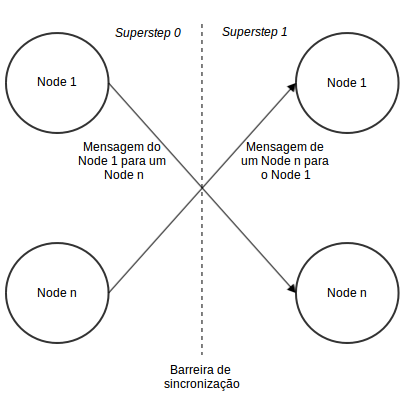
\includegraphics[width=90mm]{bspmodel.png}
	\caption{Um \textit{superstep} no modelo BSP}
 \label{fig:bspmodel}
\end{figure}

Seguindo este modelo é possível descrever algoritmos distribuídos de forma 
progressiva, tendo em consideração o possível paralelismo da solução, devido ao 
mecanismo de comunicação e de sincronização. A sincronização das entidades é  
feita entre as diversas iterações, denominadas no modelo por 
\textit{supersteps}, o que permite a troca de mensagens entre as componentes de 
processamento de uma iteração para a seguinte como se pode ver na Figura 
\ref{fig:bspmodel}.

Num ambiente distribuído deve-se ter em conta que a comunicação é normalmente 
feita através da rede, salvo exceções, nomeadamente quando o processamento 
está a ser feito no mesmo \textit{node}.

\subsection{\textit{Superstep}}
%Estas plataformas exportam uma interface programável com algumas semelhanças assim como uma típica computação de um grafo, em que consiste começar por iniciar o respetivo grafo seguido de um número variável de \textit{supersteps} (iterações) até que todos os vértices estejam inativos (não têm que participar na computação).
\textit{Supersteps} é o nome dado as iterações do modelo BSP e é onde ocorre a computação.
Durante cada \textit{superstep} é chamada (paralelamente) para cada vértice do grafo uma função definida pelo utilizador que irá delinear o seu comportamento.
Durante o processamento de um \textit{node}, tem-se acesso às mensagem que lhe foram enviadas no \textit{superstep} anterior, sendo também possível enviar mensagens, que irão ser recebidas do próximo \textit{superstep}, para outros nós.
Este modelo tem uma barreira de sincronização entre \textit{supersteps}, que faz com que cada um só se inicie após todos os nós entrarem na barreira de sincronização, fazendo com que a performance global seja afetada pelo nó que demore mais a processar.
De qualquer modo, o modelo simplifica a semântica da implementação dos algoritmos e tem normalmente um melhor desempenho que as implementações em Map Reduce devido à facilidade em que há em partilhar o estado entre os vários nós.
\import{"../hama-giraph comparison/"}{"HVSG"}
\import{"../hama-giraph comparison/"}{"ExemploGraphBSP"}